\documentclass[aspectratio=169,14pt,usenames,dvipsnames]{beamer}

\usepackage[utf8]{inputenc}
\usepackage{fontspec}
\usepackage{enumitem}
\usepackage{calc}

\usepackage{datetime}
\newcommand\builddate{%
   \ifcase \month%
        \or Janeiro%
        \or Fevereiro%
        \or Março%
        \or Abril%
        \or Maio%
        \or Junho%
        \or Julho%
        \or Agosto%
        \or Setembro%
        \or Outubro%
        \or Novembro%
        \or Dezembro%
    \fi\space\number\year%
}

\newcommand{\loadtheme}[1]{%
    \input{themes/#1}%
}
\newcommand{\presentationlanguage}[1]{%
    \usepackage[#1]{babel}%
}

\newcommand{\usecodingsamples}[1]{%
    \usepackage{listings}%
    \input{listings/#1}%
}

% Configura a apresentação para ser executada em tela cheia.
\newcommand{\setfullscreen}{\hypersetup{pdfpagemode=FullScreen}}

% Hide beamer navigation simbols
\beamertemplatenavigationsymbolsempty

%
% Standard frames
%

% coverframe
\newcommand{\coverframe}{%
    \begin{frame} %
        \titlepage %
    \end{frame} %
}

% finalframe{email}
\newcommand{\finalframe}[2][Thank you!]{%
    \begin{frame}%
        \begin{flushright}%
            \huge \textbf{#1}%
            \vfill%
            \large \textbf{#2}%
        \end{flushright}%
    \end{frame}%
}

% bigtitle{title}
\newcommand{\bigtitle}[1]{%
    \begin{frame}%
        \begin{center}%
            \Huge {#1}%
        \end{center}%
    \end{frame}%
}

% citation{cite}{author}
\renewcommand{\citation}[2]{%
    \begin{frame}%
        \begin{center}%
            \vspace{1cm}
            \large \textit{"#1"}\\%
            \vspace{1cm}
            \footnotesize {#2}%
        \end{center}%
    \end{frame}%
}

% bigimage{file}
\newcommand{\bigimage}[2][1.0]{%
    {%
        \usebackgroundtemplate{}%
        \begin{frame}%
            {%
            \makebox[\textwidth][c]{%
              \includegraphics[height=#1\paperheight, width=#1\paperwidth,%
                               keepaspectratio]{#2}%
              }%
            }%
        \end{frame}%
    }%
}


\loadtheme{photoroll}

\subtitle{Conceitos Básicos de Fotografia Digital}
\title{Composição}
\author{}
\institute{Rafael\textbf{Jeffman}\\\tiny{F O T O G R A F I A}}
\date{Abril de 2018}

\begin{document}

%01
\coverframe

%02
\begin{frame}
    \frametitle{Composição}
    \begin{itemize}
      \item "Compor, é o ato de dar forma ao unir ou combinar diferentes elementos,
      partes ou ingredientes." (David Präkel)
      \item Compor é o ato de organizar os elementos de uma obra, decidindo como
      as partes interagem, o que é mostrado, o que é oculto.
    \end{itemize}
\end{frame}

%03
\begin{frame}
    \frametitle{Por que Compor?}
    \begin{itemize}
      \item Vemos uma cena com nosso cérebro, não com nossos olho.
      \item Dessa forma, enxergamos a cena de forma diferente da câmera.
      \item Quando vemos uma cena, além da imagem, sentimos a cena, usamos a emoção.
      \item Quando uma câmera "vê" uma cena, não tem emoção, apenas a imagem.
      \item O mais difícil na composição é compor como a vemos, e não como pensamos em vê-la.
    \end{itemize}
\end{frame}

%04
\begin{frame}
    \frametitle{Visualizando a Imagem}
    \begin{itemize}
      \item Qual a finalidade de uma imagem fotográfica?
      \item Qual a mensagem quero passar com essa fotografia?
      \item O que mostrar numa imagem? O que esconder?
      \item A composição de uma imagem constitui na organização de linhas, formas,
      cores, texturas, e padrões.
    \end{itemize}
\end{frame}

%05
\begin{frame}
    \frametitle{O Fotograma}
    \begin{itemize}
      \item Enxergamos o mundo sem limites.
      \item Na fotografia, o fotograma é o limite do que a câmera consegue ver.
      \item O quadro do fotograma, limita o \textit{quadro} que podemos registrar do mundo.
      \item Existem suportes fotográficos de diversos aspectos, sendo os mais comuns o 3x2 e o 4x3.
      \item Podemos alterar o quadro da imagem, por corte, ou por composição, como nas panorâmicas.
    \end{itemize}
\end{frame}

%06
\begin{frame}
    \frametitle{Redução da Dimensionalidade}
    Outro efeito importante da fotografia é a redução da dimensionalidade com que vemos o mundo,
    de um mundo com três dimensões para uma representação em duas dimensões.
\end{frame}

%07
\begin{frame}
    \frametitle{Razão Áurea}
    \begin{itemize}
      \item O "número de ouro", \textit{phi}, 1.618034, era considerado a chave
      para a matemática divina.
      \item A \textbf{razão áurea}, é uma divisão baseada na proporção do número de ouro.
      \item Compor, utilizando a razão áurea, agrada instintivamente.
      \item Obviamente, nem todo objeto é adequado a esse tipo de composição.
    \end{itemize}
\end{frame}

%08
\bigimage{images/golden-ratio.png}
%09
\bigimage{images/ex-golden-ratio.jpg}

%10
\begin{frame}
    \frametitle{Espiral de Fibonacci}
    \begin{itemize}
      \item Conhecida desde 200 A.C., e popularizada no ocidente for Leonardo de Pisa (Fibonacci),
      a sequência de Fibonacci aparece em diversos elementos na natureza.
      \item Podemos criar uma espiral com os números de Fibonacci: 1, 1, 2, 3, 5, 8, 13, 21, 34, 55, 89...
      \item Essa composição no quadro também é agradável ao observador.
    \end{itemize}
\end{frame}

%11
\bigimage{images/fibonacci-spiral.png}
%12
\bigimage{images/ex-fibonacci-spiral-01.jpg}
%13
\bigimage{images/ex-fibonacci-spiral-02.jpg}

%14
\begin{frame}
    \frametitle{Simetria Dinâmica}
    \begin{itemize}
      \item É uma alternativa para organizar os pontos de interesse.
      \item Baseada na simetria da razão áurea, mas utiliza diagonais para determinar os pontos.
      \item É mais fácil de visualizar que a proporção áurea.
      \item Os pontos são criados a partir de uma diagonal de um canto do fotograma formando 90$^o$
      com a diagonal principal oposta.
    \end{itemize}
\end{frame}

%15
\bigimage{images/simetria-dinamica.png}
%16
\bigimage{images/ex-simetria-dinamica.jpg}

%17
\begin{frame}
    \frametitle{Regra dos Terços}
    \begin{itemize}
      \item A \textbf{regra dos terços} é uma simplificação da razão áurea.
      \item É a regra mais utilizada na fotografia.
      \item Divide-se a imagem em três partes iguais, na horizontal e na vertical.
      \item Embora seja muito útil, cria um resultado de menor impacto que as outras regras.
    \end{itemize}
\end{frame}

%18
\bigimage{images/rule-of-thirds.jpg}
%19
\bigimage{images/ex-rule-of-thirds.jpg}

%20
\begin{frame}
    \frametitle{Linhas}
    \begin{itemize}
      \item Linhas são utilizadas para orientar os olhos dentro da foto.
      \item As linhas podem ser reais, ou virtuais (como uma pessoa olhando para outra).
      \item Tendemos a acompanhar linhas horizontais e diagonais, e somos bloqueados por linhas verticais.
      \item Utilizar um \textit{ponto de fuga} dentro da foto ajuda a direcionar o olhar.
    \end{itemize}
\end{frame}

%21
\begin{frame}
    \frametitle{Diagonais}
    \begin{itemize}
      \item Linhas horizontas e verticais trazem equilíbrio e deixam a foto mais "estática".
      \item Diagonais trazem movimento e dinamicidade para a foto.
      \item O uso de linhas diagonais acentua o movimento em uma foto.
    \end{itemize}
\end{frame}

%22
\begin{frame}
    \frametitle{Quadros}
    \begin{itemize}
      \item Utilize quadros naturais dentro da foto para destacar objetos.
      \item Mesmo quando o quadro não é claro, a nossa tendência é fechar, instintivamente,
      formas geométricas.
      \item Quadros dentro da imagem ajudam a organizar e separar os elementos.
    \end{itemize}
\end{frame}

%23
\begin{frame}
    \frametitle{\Large Contraste entre o Objeto e o Fundo}
    \begin{itemize}
      \item Procure separar o objeto do entorno.
      \item Podemos fazer isso utilizando o foco seletivo (grande abertura de diafragma).
      \item Mova-se em torno do objeto, procurando novos ângulos.
      \item Reposicione o objeto, para destacá-lo do fundo.
    \end{itemize}
\end{frame}

%24
\begin{frame}
    \frametitle{Preencha o Quadro}
    \begin{itemize}
      \item Preencha o quadro com o objetivo da sua foto.
      \item Chegue mais perto do objeto.
    \end{itemize}
    \begin{center}
      "If your pictures aren’t good enough, you’re not close enough." (Robert Capa)
    \end{center}
\end{frame}

%25
\begin{frame}
    \frametitle{Centralize o Olho Dominante}
    \begin{itemize}
      \item Em retratos, o foco deve, sempre, estar nos olhos do retratado.
      \item Se os olhos não estão no mesmo plano, o olho mais próximo deve estar em foco.
      \item Posicione o olho dominante na linha central do quadro.
      \item Isso dará a impressão que o retrato está olhando de volta.
    \end{itemize}
\end{frame}

%26
\begin{frame}
    \frametitle{Padrões e Repetição}
    \begin{itemize}
      \item Utilize padrões repetitivos para uma composição agradável.
      \item Padrões repetitivos ditam o \textit{ritmo} da foto.
      \item Uma quebra no padrão adiciona tensão e interesse.
    \end{itemize}
\end{frame}

%27
\begin{frame}
    \frametitle{Simetria}
    \begin{itemize}
      \item A simetria traz conforto e equilíbrio.
      \item Utilize a simetria para fotos que transmitam um forte senso de estrutura, equilíbrio.
      \item A simetria pode ser cansativa, pela falta de tensão na foto.
    \end{itemize}
\end{frame}

%28
\begin{frame}
    \frametitle{Steve McCurry}
    \begin{itemize}
      \item Steve McCurry é o autor da foto \textbf{Menina Afegã}, possivelmente a foto mais
      reproduzida da história.
      \item É um dos fotógrafos mais conhecidos da história, e suas fotos são bastante
      rígidas do ponto de vista de composição.
      \item McCurry possui diversos vídeos onde fala sobre conceitos de composição de
      forma bastante acessível.
      \item \url{https://www.youtube.com/watch?v=7ZVyNjKSr0M}
    \end{itemize}
\end{frame}

%29
\begin{frame}
    \frametitle{Percepção da Gestalt}
    \begin{itemize}
      \item A \textit{psicologia da Gestalt} foi fundada na Áustria e na Alemanha,
      no início do século XX.
      \item Tem por princípio que o todo é maior que a soma das partes.
      \item Embora a Gestalt tenha adaptado suas teorias à pesquisa experimental,
      oferece algumas observações interessantes a respeito do processo de percepção.
    \end{itemize}
\end{frame}

%30
\begin{frame}
    \frametitle{Princípios e Leis da Gestalt}
    \begin{itemize}
      \item A \textit{Gestalt} é regida por princípios e leis.
      \item Os princípios e leis da Gestalt trazem a ideia de reagrupar e reestruturar
      os elementos visuais para que "façam sentido" quando vemos a imagem inteira.
      \item Podemos utilizar a Gestalt para acelerar ou diminuir a velocidade com que
      reconhecemos os elementos. Na fotografia, muitas vezes queremos diminuir a
      velocidade, ao contrário de gráficos e diagramas.
    \end{itemize}
\end{frame}

% %31
\begin{frame}
    \frametitle{Leis da Gestalt}
    \begin{itemize}
      \item[1.] Lei da Proximidade: elementos visuais próximos são agrupados.
      \item[2.] Lei da Semelhança: elementos visuais semelhantes, tendem a ser agrupados.
      \item[3.] Lei do Fechamento: elementos arranjados mais ou menos como uma forma,
      são vistos como formando a forma; a mente busca completude.
    \end{itemize}
\end{frame}

%32
\begin{frame}
    \frametitle{Leis da Gestalt}
    \begin{itemize}
      \item[4.] Lei da Simplicidade: a mente busca explicações visuais simples.
      \item[5.] Lei do Destino Comum: assume-se que elementos agrupados movem-se como um só.
      \item[6.] Lei da Continuidade: a mente faz com que linhas e formas continuem além de suas extremidades.
      \item[7.] Lei da Segregação: para que uma figura seja percebida, deve destacar-se de seu fundo.
    \end{itemize}
\end{frame}

%33
\begin{frame}
    \frametitle{Princípios da Gestalt}
    {\textbf{\large Emergência}}
    \vspace{1cm}

    Partes de uma imagem que não contém informação suficiente para explicá-la,
    emergem como resultado de visualização por tempo suficientemente longo.
\end{frame}

%34
\begin{frame}
  \frametitle{Princípios da Gestalt}
  {\textbf{\large Reificação}}
  \vspace{1cm}

  A mente preenche uma forma ou área devido a dados visuais inadequados. Isso
  inclui a lei de fechamento.
\end{frame}

%35
\begin{frame}
  \frametitle{Princípios da Gestalt}
  {\textbf{\large Multi-estabilidade}}
  \vspace{1cm}

  Em alguns casos, quando há indicações suficientes de profundidade, um objeto
  pode ser visto como que se invertendo espontaneamente (ex.: M. C. Escher,
  Salvador Dalí). Dificilmente é explorado na fotografia.
\end{frame}

%36
\begin{frame}
  \frametitle{Princípios da Gestalt}
  {\textbf{\large Invariância}}
  \vspace{1cm}

  Objetos podem ser reconhecidos, apesar da orientação, rotação, aspecto, escala
  ou outros fatores.
\end{frame}

%37
\bigtitle{\textbf{Conheça as regras.\\Use as regras.\\Quebre as regras.}}

%38
\citation{Consultar as regras de composição antes de fazer uma fotografia
é quase como consultar as leis de gravitação antes de sair para caminhar.}{Edward Weston}

%39
\bigtitle{exemplos}

%40
\bigimage{images/corte.jpg}

%41
\bigimage{images/foco.jpg}

%42
\bigimage[2.0]{images/foco.jpg}

%43
\begin{frame}
    \frametitle{Compare as Imagens}
    \begin{columns}
      \column{0.45\paperwidth}
        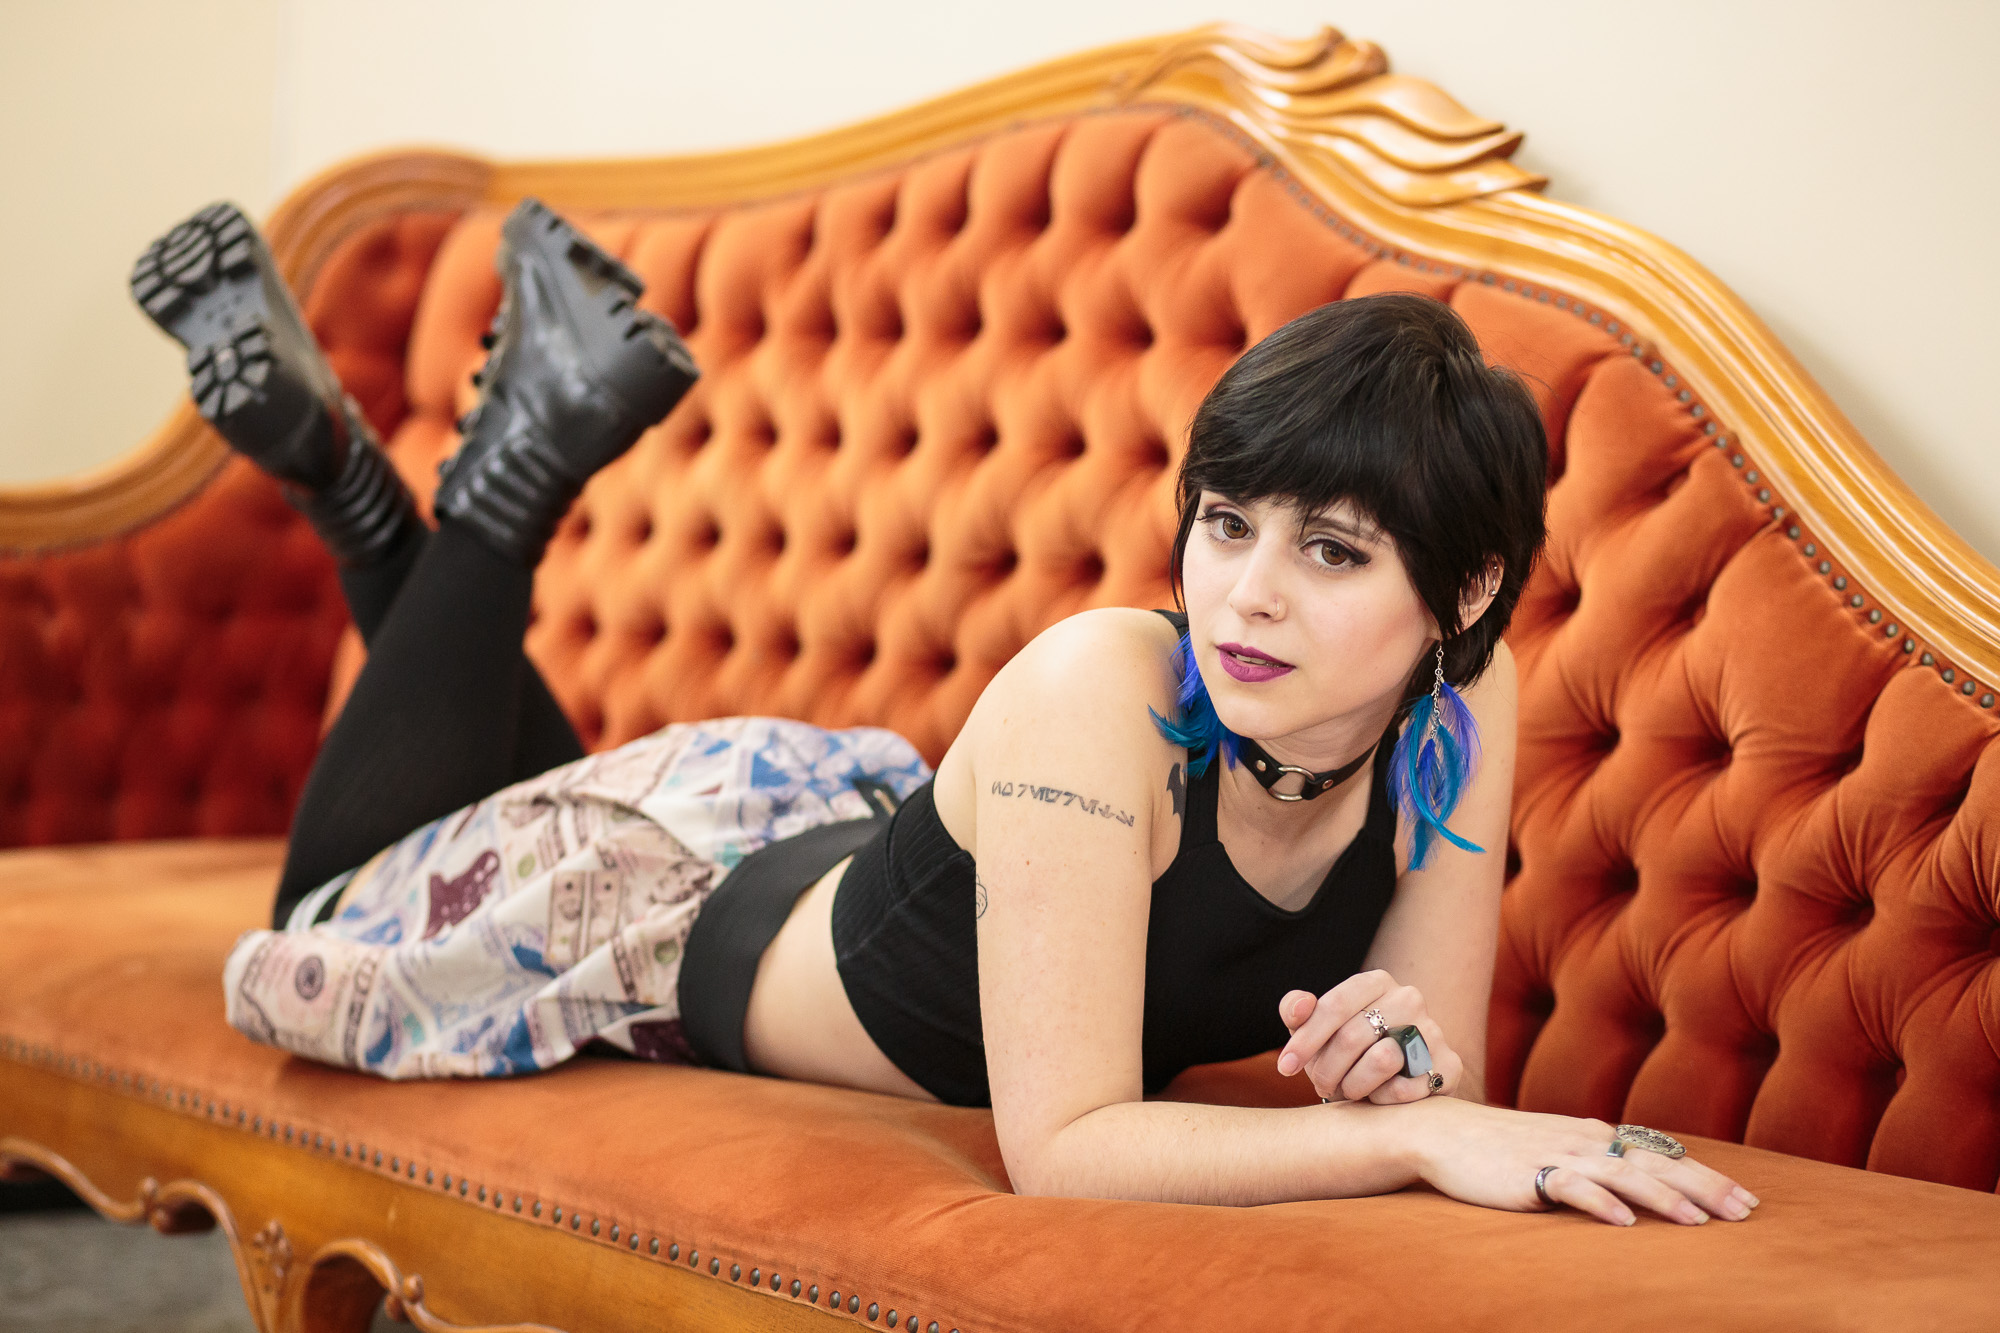
\includegraphics[width=0.45\paperwidth]{images/equilibrio_1.jpg}
      \column{0.45\paperwidth}
        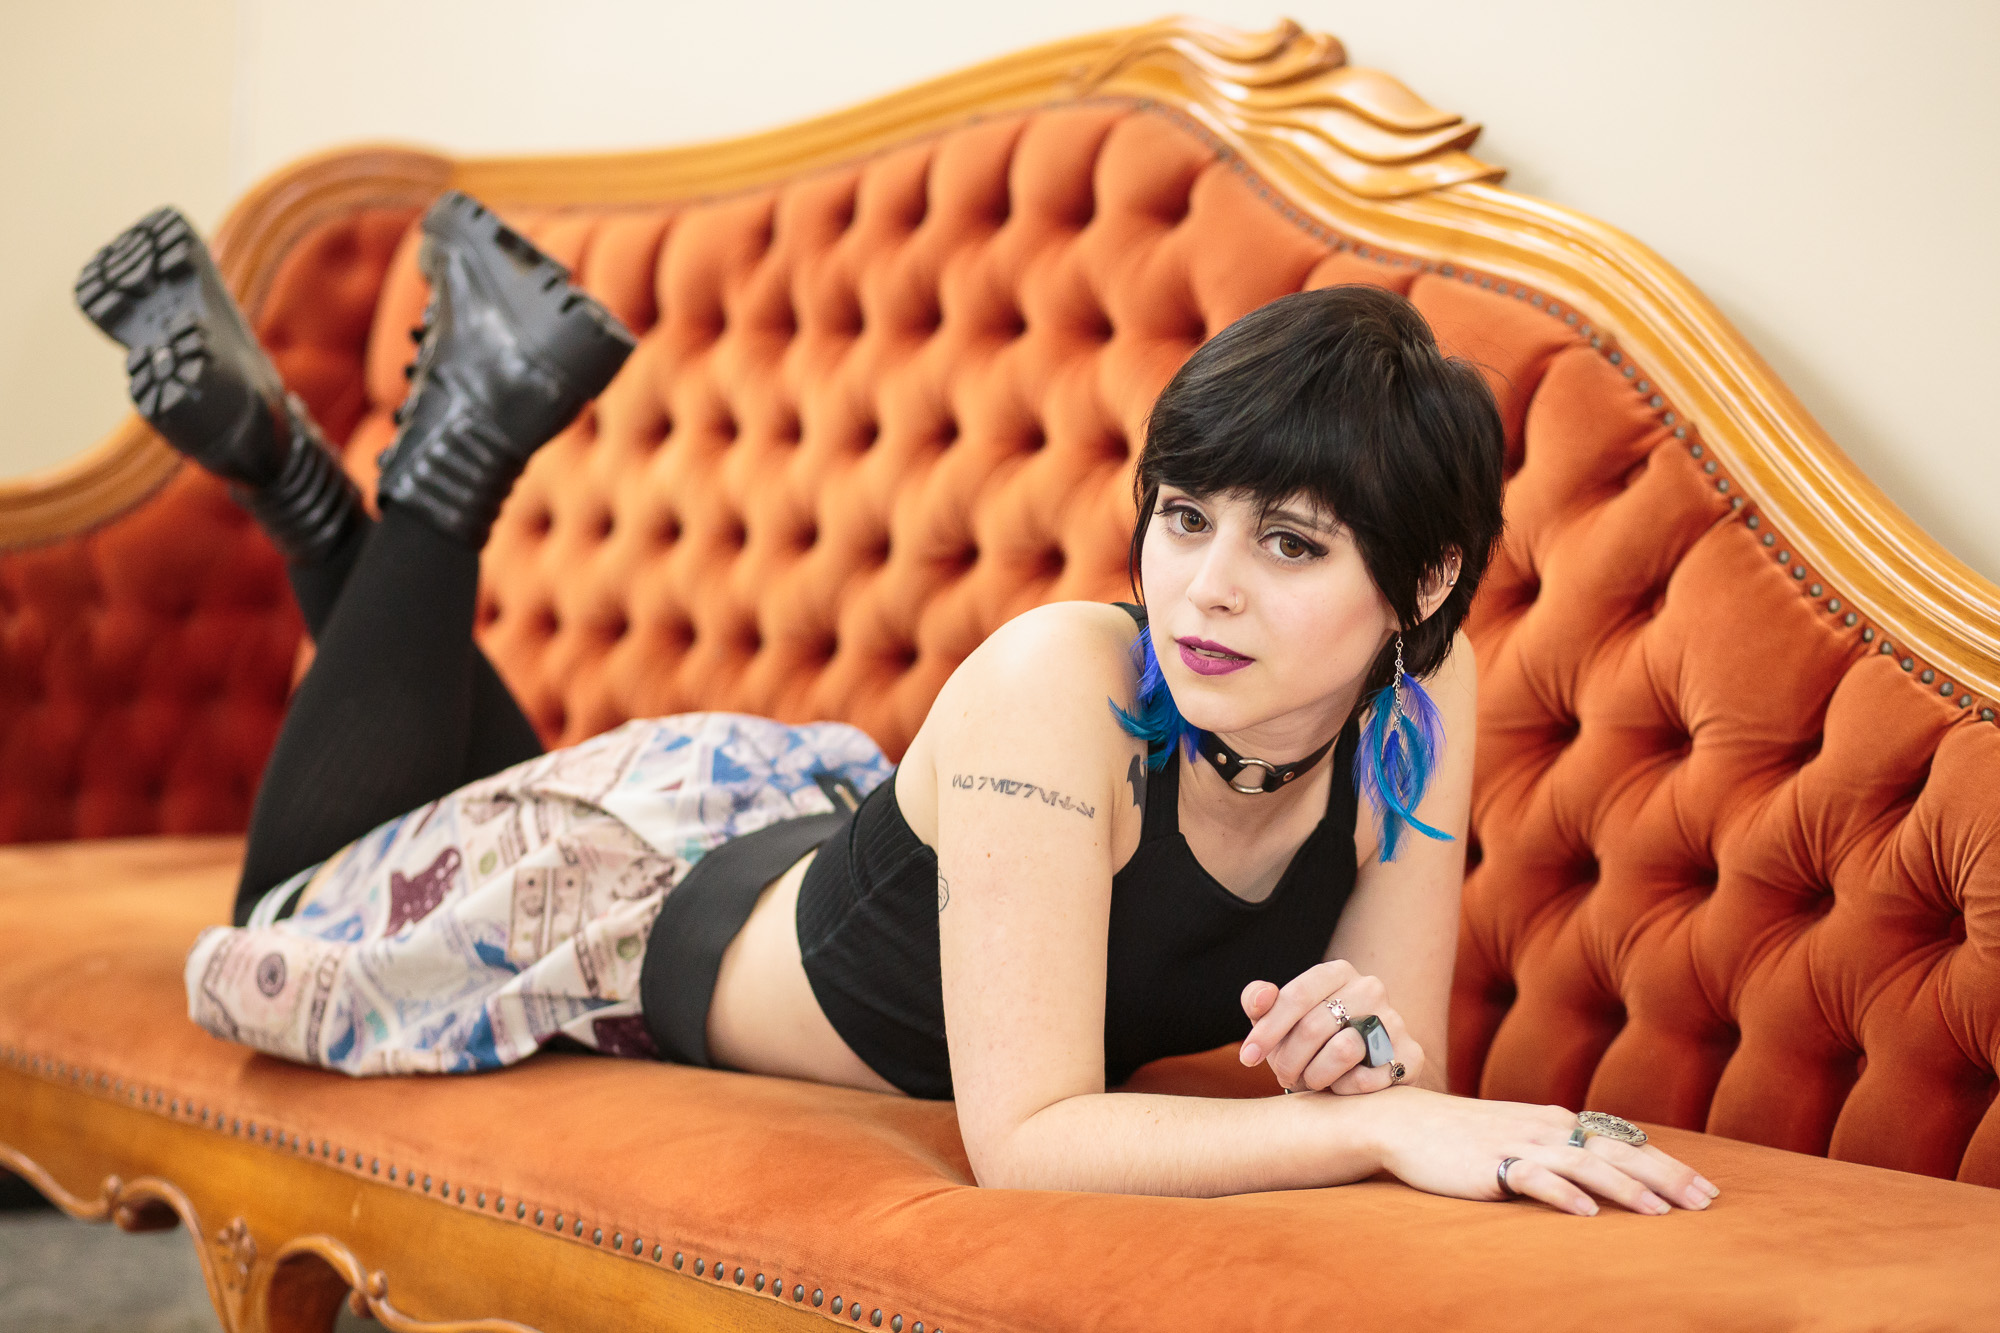
\includegraphics[width=0.45\paperwidth]{images/equilibrio_2.jpg}
    \end{columns}
\end{frame}

%44
\bigimage{images/equilibrio_1.jpg}

%45
\bigimage{images/equilibrio_2.jpg}

%46
\finalframe[Vamos gastar o obturador!]{rafasgj@gmail.com}

%47
\begin{frame}
    \frametitle{Bibliografia}
    \begin{itemize}
      \item \textbf{O Olho do Fotógrafo}. Michael Freeman. Bookman, 2012.
      \item \textbf{Composição}. David Präkel. Bookman, 2010.
      \item \textbf{O novo manual de Fotografia}. John Hedgecoe. Senac, 2005.
    \end{itemize}
\end{frame}

\end{document}
